\documentclass{article}


\usepackage[utf8]{inputenc}
\usepackage[top=0.5in, bottom=0.5in, left=0.5in, right=0.5in]{geometry}

%%%%% IMÁGENES %%%%%
\usepackage{watermark}
\usepackage{graphicx} 
\usepackage{wrapfig}

%%%%% SEPARACIÓN E IDENTACIÓN EN LOS PÁRRAFOS %%%%%
\setlength{\parindent}{0em}
\setlength{\parskip}{0.4em}

%%%%%% Symbols square %%%%%%
\usepackage{amsfonts}
\usepackage{amssymb}

\usepackage[dvipsnames]{xcolor}
\usepackage[hidelinks]{hyperref}


\usepackage{watermark}
%%% Funciones %%%

\begin{document}
\thispagestyle{empty} 
%\begin{wrapfigure}{lt}{0.3\textwidth}
%  \centering
%  
\includegraphics[width=0.30\textwidth]{pheto.jpg}
%\end{wrapfigure}
\begin{minipage}{0.4\linewidth}
\textbf{\huge{Isaac Lacort Magán}}
\vspace{0.2cm}

\large{\color{BlueViolet}Software Developer}
\end{minipage}
\hspace{1cm}
\begin{minipage}{0.5\linewidth}
\end{minipage}
\vspace{1.25cm}

\thiswatermark{\centering \put(440,-105){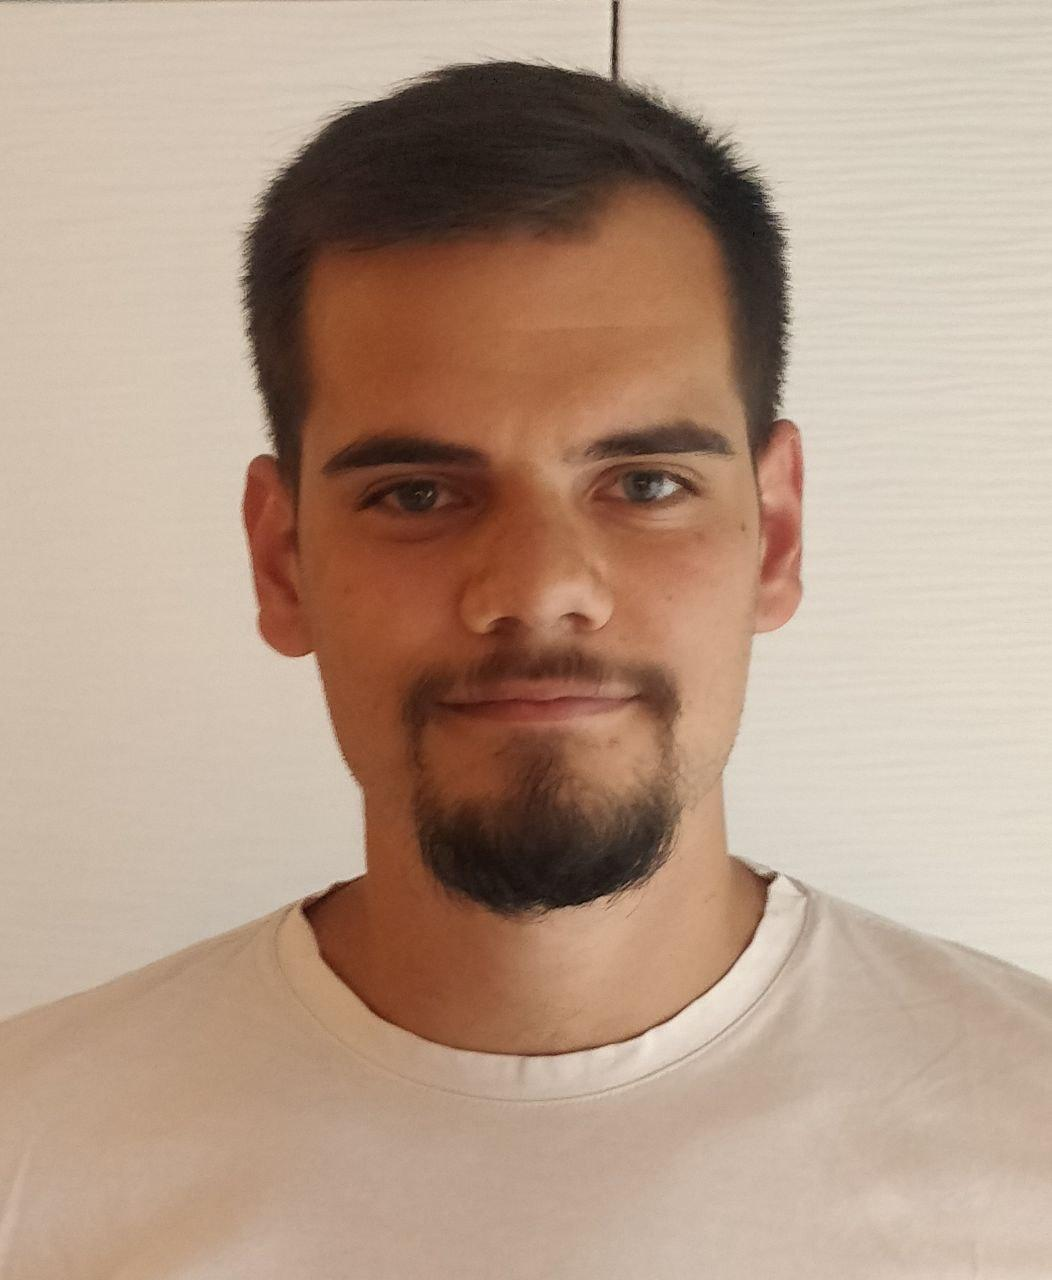
\includegraphics[width=3cm]{pheto2.jpg}} }

\begin{minipage}[t]{0.3\linewidth}
  
  \setlength{\parskip}{0.3em}
  \textbf{\Large{\color{BlueViolet}Personal Info}}\\[-0.25cm]
  {\color{BlueViolet} \rule{\linewidth}{0.1mm} } \\[-0.25cm]
  \textbf{\large{DNI}} \hfill 51147166-L
  \vspace{0.1cm}
  
  \textbf{\large{Phone}} \hfill 622 700 374
  \vspace{0.1cm}

  \textbf{\large{E-mail}} \hfill isaaclacort@gmail.com
  \vspace{0.1cm}

  \textbf{\large{Address}}\\  
  \normalsize C/ Cenicienta, 8, portal C, 3ºD \\[0.06cm]
  \normalsize 28018 Madrid
  \vspace{0.1cm}
  
  \textbf{\large{LinkedIn}}\\
  \href{https://www.linkedin.com/in/isaac-lacort-706725168/}{\textcolor{blue}{\underline{linkedin.com/in/isaac-lacort}}}
  
  \vspace{0.3cm}
  \textbf{\Large{\color{BlueViolet}Soft Skills}}\\[-0.25cm]
  {\color{BlueViolet} \rule{\linewidth}{0.1mm} }\\[-0.25cm]
  Abstract Thinking 

  Attention to Detail

  Teamwork

  Creativity
  
  \vspace{0.3cm}
  \textbf{\Large{\color{BlueViolet}Software}}\\[-0.25cm]
  {\color{BlueViolet} \rule{\linewidth}{0.1mm} }\\
  \large Linux \hfill $\color{blue} \blacksquare\color{blue} \blacksquare \color{blue} \blacksquare \color{gray} \blacksquare  \color{gray} \blacksquare$  \\[-0.8mm]
  \null\hfill \small{ $\color{blue} \textnormal{good}$}

  \large Eclipse \hfill $\color{blue} \blacksquare\color{blue} \blacksquare \color{blue} \blacksquare \color{gray} \blacksquare  \color{gray} \blacksquare$  \\[-0.8mm]
  \null\hfill \small{ $\color{blue} \textnormal{good}$}

  \large Android Studio \hfill $\color{blue} \blacksquare\color{blue} \blacksquare \color{gray} \blacksquare \color{gray} \blacksquare  \color{gray} \blacksquare$  \\[-0.8mm]
  \null\hfill \small{ $\color{blue} \textnormal{familiar}$}

  \large Spring Boot \hfill $\color{blue} \blacksquare\color{gray} \blacksquare \color{gray} \blacksquare \color{gray} \blacksquare  \color{gray} \blacksquare$  \\[-0.8mm]
  \null\hfill \small{ $\color{blue} \textnormal{basic}$}

  \large Git \hfill $\color{blue} \blacksquare\color{blue} \blacksquare \color{blue} \blacksquare \color{blue} \blacksquare  \color{gray} \blacksquare$  \\[-0.8mm]
  \null\hfill \small{ $\color{blue} \textnormal{very good}$}

  \large Docker \hfill $\color{blue} \blacksquare\color{blue} \blacksquare \color{gray} \blacksquare \color{gray} \blacksquare  \color{gray} \blacksquare$  \\[-0.8mm]
  \null\hfill \small{ $\color{blue} \textnormal{familiar}$}

  \large MySQL \hfill $\color{blue} \blacksquare\color{blue} \blacksquare \color{gray} \blacksquare \color{gray} \blacksquare  \color{gray} \blacksquare$  \\[-0.8mm]
  \null\hfill \small{ $\color{blue} \textnormal{familiar}$}

  \large SQLite \hfill $\color{blue} \blacksquare\color{gray} \blacksquare \color{gray} \blacksquare \color{gray} \blacksquare  \color{gray} \blacksquare$  \\[-0.8mm]
  \null\hfill \small{ $\color{blue} \textnormal{basic}$}

  \vspace{0.3cm}
  \textbf{\Large{\color{BlueViolet}Programming}}\\[-0.25cm]
  {\color{BlueViolet} \rule{\linewidth}{0.1mm} }\\
  \large Java \hfill $\color{blue} \blacksquare\color{blue} \blacksquare \color{blue} \blacksquare \color{blue} \blacksquare  \color{gray} \blacksquare$  \\[-0.8mm]
  \null\hfill \small{ $\color{blue} \textnormal{very good}$}

  \large Python \hfill $\color{blue} \blacksquare\color{blue} \blacksquare \color{gray} \blacksquare \color{gray} \blacksquare  \color{gray} \blacksquare$  \\[-0.8mm]
  \null\hfill \small{ $\color{blue} \textnormal{familiar}$}

  \large C \hfill $\color{blue} \blacksquare \color{blue} \blacksquare \color{gray} \blacksquare \color{gray} \blacksquare  \color{gray} \blacksquare$  \\[-0.8mm]
  \null\hfill \small{ $\color{blue} \textnormal{familiar}$}

  \large Haskell \hfill $\color{blue} \blacksquare \color{gray} \blacksquare \color{gray} \blacksquare \color{gray} \blacksquare  \color{gray} \blacksquare$  \\[-0.8mm]
  \null\hfill \small{ $\color{blue} \textnormal{basic}$}

  \textbf{\Large{\color{BlueViolet}Languages}}\\[-0.25cm]
  {\color{BlueViolet} \rule{\linewidth}{0.1mm} }\\
  \large Spanish \hfill $\color{blue} \blacksquare\color{blue} \blacksquare \color{blue} \blacksquare \color{blue} \blacksquare  \color{blue} \blacksquare$  \\[-0.8mm]
  \null\hfill \small{ $\color{blue} \textnormal{native}$}

  \large English \hfill $\color{blue} \blacksquare\color{blue} \blacksquare \color{blue} \blacksquare \color{gray} \blacksquare  \color{gray} \blacksquare$  \\[-0.8mm]
  \null\hfill \small{ $\color{blue} \textnormal{intermediate}$}
  
\end{minipage}
\hspace{0.25cm}\vline\hspace{0.25cm}
\begin{minipage}[t]{0.66\linewidth}
  \setlength{\parskip}{0.3em}

  \textbf{\Large{\color{BlueViolet}Experience}}\\[-0.25cm]
  {\color{BlueViolet} \rule{\linewidth}{0.1mm} }\\[-0.05cm]
  \begin{tabular}{l l}
    \multicolumn{2}{p{6cm}}{\hspace{0.40cm} \textbf{Android App Developer}}\\[0.1cm]
    2019 & \textbf{Colaboration Internship} (3 months)\\
         & \textbf{Universidad Politecnica de Madrid (UPM)} \\
         & \multicolumn{1}{p{11cm}}{DynApp development, an Android app which purpose is to measure the vibrations to which structures such as beams or bridges are subjected to in order to analyze their stability. To do so, the app stores and analyzes the data collected by the smartphone's accelerometer placed over one of these structures. The purpose of the analysis is to calculate the Discrete Fourier Transform (DFT), which can give us information about whether a structure has been damaged. My job consisted on the development of the entire app and the contribution to the deployment of numerous analysis algorithms, such as an interpolation algorithm to preprocess the data before calculating the DFT.}\\ \\[-0.1cm]
    \multicolumn{2}{p{6cm}}{\hspace{0.40cm} \textbf{Software Developer}}\\[0.1cm]
    2019 & \textbf{Summer Internship GMV} (2 months)\\
         & \multicolumn{1}{p{11cm}}{Project P3-NEO-XII. Development of the file subsystem of satelite images for the installation in a telescope in an extreme environment. My job consisted on separating the program in different modules, one for each tool that it used. The tools the program used were Apache Tomcat, PostgreSQL and RabbitMQ. I created a container for each module and connected the Tomcat's container to the others.} \\
  \end{tabular}
  \vspace{0.3cm}
  
  \textbf{\Large{\color{BlueViolet}Education}}\\[-0.25cm]
  {\color{BlueViolet} \rule{\linewidth}{0.1mm} }\\[-0.25cm]
  \begin{tabular}{l l}
    \multicolumn{1}{p{0.6cm}}{2016-now}& \multicolumn{1}{p{8.4cm}}{\textbf{Degree in Mathematics and Computer Science, Universidad Politécnica de Madrid} }\\
         & \normalsize \quad $92.5\%$ ECTS passed.\\
            & \normalsize \quad $21.25\%$ ECTS passed cum laude.\\
         & \normalsize \quad GPA: $8.34/10$ \\[0.3cm]
    2018 & \textbf{Workshop SAMSUNG-UPM (100 hours):} \\ & \textbf{Introduction to Android App Development} \\
         & \multicolumn{1}{p{11cm}}{\normalsize We were introduced to basic app development and Android Studio Environment. I learnt about the Android app lifecycle, app elements such as activities, manifest and gradle scripts; services, SQLite and basic material design elements like listview, recicler view, menu and toolbar among others.} \\ \\[-0.12cm]
    2018 & \textbf{Workshop SAMSUNG-UPM (75 hours):} \\ & \textbf{Android's Advanced Development} \\
         & \multicolumn{1}{p{11cm}}{\normalsize We implemented applications that used web services. To do so we were introduced to the libraries OkHttp, Retrofit, Volley and Picasso.} \\
  \end{tabular}
  \vspace{0.3cm}
  
  \textbf{\Large{\color{BlueViolet}Interests}}\\[-0.25cm]
  {\color{BlueViolet} \rule{\linewidth}{0.1mm} }\\[-0.25cm]
  Computational Topology applied to clustering techniques.

  Functional Programming

  Software Development

  Formal methods and critical systems

  
\end{minipage}
\end{document}

%%% Local Variables:
%%% mode: latex
%%% TeX-master: t
%%% End:
